\documentclass[12pt]{article}

% TEMPLATE DEFAULT PACKAGES
\usepackage{amssymb,amsmath,amsfonts,eurosym,geometry,ulem,graphicx,color,setspace,sectsty,comment,natbib,pdflscape,array,adjustbox}

% ADDED PACKAGES FOR THIS MANUSCRIPT
\usepackage{palatino,newtxmath,multirow,titlesec,threeparttable,tabu,booktabs,titlesec,threeparttable,mathtools,bm,bbm,subcaption,pdflscape,tcolorbox,mathrsfs}
% endfloat,

\usepackage{afterpage}
\usepackage[hyphens]{url}
\usepackage[margin=1cm]{caption}

\usepackage[draft]{hyperref}
\newcommand{\tim}{$\,\times\,$}
% FIGURES & TABLES CAPTION STYLING
\captionsetup[figure]{labelfont={bf},name={Figure},labelsep=period}
\captionsetup[table]{labelfont={bf},name={Table},labelsep=period}

% SECTION TITLE SETTINGS
\titlelabel{\thetitle.\enskip}
\titleformat*{\section}{\large\bfseries}
\titleformat*{\subsection}{\normalsize\bfseries}

% COLUMN TYPES
\newcolumntype{L}[1]{>{\raggedright\let\newline\\\arraybackslash\hspace{0pt}}m{#1}}
\newcolumntype{C}{>{\centering\arraybackslash}p{5.2em}}
\newcolumntype{D}{>{\centering\arraybackslash}p{5em}}
\newcolumntype{R}[1]{>{\raggedleft\let\newline\\\arraybackslash\hspace{0pt}}m{#1}}


% MARGINS AND SPACING
\normalem
\geometry{left=1.1in,right=1.1in,top=1.0in,bottom=1.0in}
\setlength{\parskip}{2.5pt}

% SPECIAL CELL 
\newcommand{\specialcell}[2][c]{%
	\begin{tabular}[#1]{@{}l@{}}#2\end{tabular}}

% NO INDENT ON FOOTNOTES
\usepackage[hang,flushmargin]{footmisc}

\begin{document}






\afterpage{%
  \clearpage% 
\begin{landscape}
{\footnotesize
\begin{table}[]
\small
\centering
\caption{Census Household-level Estimates }\label{table:censusestimates}
\vspace{-2mm}
\begin{tabular}{lDDDDDDDD}
\toprule
 & \small (1) & \small (2)  & \small (3) & \small (4) & \small (5)  & \small (6)  & \small (7) & (8)\\
 & \small Flush Toilet & \small Water Indoors  & \small Electricity Cooking & \small Electricity Heating & \small Electricity Lighting  & \small Number of Rooms  & \small Household Size & Population Density\\ \midrule 
inside project      &       0.097                   &       0.182\textsuperscript{a}&       0.182\textsuperscript{a}&       0.163\textsuperscript{a}&       0.107                   &       0.069                   &       0.070                   &    -813.497                   \\
                    &     (0.069)                   &     (0.046)                   &     (0.064)                   &     (0.062)                   &     (0.066)                   &     (0.169)                   &     (0.079)                   &  (1228.688)                   \\[0.55em]
0-300m outside project &      -0.042                   &       0.015                   &      -0.015                   &      -0.003                   &      -0.025                   &      -0.092                   &      -0.094\textsuperscript{c}&     385.617                   \\
                    &     (0.036)                   &     (0.038)                   &     (0.034)                   &     (0.036)                   &     (0.032)                   &     (0.119)                   &     (0.054)                   &   (647.578)                   \\[0.5em]
300-600m outside project &      -0.033                   &       0.009                   &      -0.015                   &      -0.001                   &      -0.017                   &      -0.093                   &      -0.048                   &    -247.696                   \\
                    &     (0.027)                   &     (0.033)                   &     (0.027)                   &     (0.029)                   &     (0.026)                   &     (0.109)                   &     (0.052)                   &   (694.350)                   \\[0.5em]
Mean Outcome 2001   &        0.79                   &        0.35                   &        0.66                   &        0.62                   &        0.77                   &        3.30                   &        3.51                   &    8,566.83                   \\
Mean Outcome 2011   &        0.83                   &        0.54                   &        0.81                   &        0.72                   &        0.82                   &        3.56                   &        3.18                   &    9,823.82                   \\
R$^2$               &       0.402                   &       0.414                   &       0.491                   &       0.474                   &       0.442                   &       0.475                   &       0.496                   &       0.458                   \\
\# projects         &         314                   &         314                   &         314                   &         314                   &         314                   &         314                   &         314                   &         314                   \\
N project areas     &       3,657                   &       3,657                   &       3,657                   &       3,657                   &       3,657                   &       3,651                   &       3,657                   &       3,657                   \\
N spillover areas   &       4,200                   &       4,200                   &       4,200                   &       4,200                   &       4,200                   &       4,192                   &       4,199                   &       4,201                   \\
N                   &      12,732                   &      12,732                   &      12,732                   &      12,732                   &      12,732                   &      12,709                   &      12,730                   &      12,734                   \\

\bottomrule
\multicolumn{9}{l}{\footnotesize All regressions include project Fixed-Effects. Standard errors clustered at the project level in parenthesis. \textsuperscript{c} p$<$0.10,\textsuperscript{b} p$<$0.05,\textsuperscript{a} p$<$0.01 }
\end{tabular}
\end{table}
}
\end{landscape}
}

\afterpage{%
  \clearpage% 
\begin{landscape}
{\footnotesize
\begin{table}[]
\small
\centering
\caption{Census Household-level Estimates }\label{table:censusestimates}
\vspace{-2mm}
\begin{tabular}{lDDDDDDDD}
\toprule
 & \small (1) & \small (2)  & \small (3) & \small (4) & \small (5)  & \small (6)  & \small (7) & (8)\\
 & \small Flush Toilet & \small Water Indoors  & \small Electricity Cooking & \small Electricity Heating & \small Electricity Lighting  & \small Number of Rooms  & \small Household Size & Population Density\\ \midrule 
\textbf{Greenfield} \\   inside project      &      -0.033                   &       0.131                   &       0.073                   &       0.035                   &       0.024                   &       0.251                   &       0.200                   &    3790.441\textsuperscript{c}\\
                    &     (0.131)                   &     (0.123)                   &     (0.111)                   &     (0.112)                   &     (0.126)                   &     (0.367)                   &     (0.209)                   &  (2196.802)                   \\[0.01em]
0-300m outside project &      -0.054                   &       0.077                   &       0.014                   &       0.036                   &      -0.030                   &       0.565\textsuperscript{c}&       0.257\textsuperscript{b}&    3716.468                   \\
                    &     (0.089)                   &     (0.091)                   &     (0.060)                   &     (0.069)                   &     (0.057)                   &     (0.287)                   &     (0.125)                   &  (2418.104)                   \\[0.01em]
300-600m outside project&       0.017                   &      -0.025                   &       0.086\textsuperscript{c}&       0.078                   &       0.096\textsuperscript{b}&       0.207                   &       0.126                   &    -466.573                   \\
                    &     (0.060)                   &     (0.076)                   &     (0.044)                   &     (0.059)                   &     (0.042)                   &     (0.195)                   &     (0.102)                   &  (1702.631)                   \\[0.8em] 
\textbf{In-Situ Upgrading} \\   inside project      &       0.320\textsuperscript{a}&       0.217\textsuperscript{b}&       0.347\textsuperscript{a}&       0.379\textsuperscript{a}&       0.220\textsuperscript{b}&       0.322                   &       0.169                   &   -3307.188                   \\
                    &     (0.111)                   &     (0.096)                   &     (0.090)                   &     (0.082)                   &     (0.095)                   &     (0.267)                   &     (0.128)                   &  (3071.103)                   \\[0.01em]
0-300m outside project &       0.018                   &       0.014                   &       0.069                   &       0.093                   &       0.026                   &      -0.250                   &      -0.012                   &    -919.031                   \\
                    &     (0.079)                   &     (0.079)                   &     (0.070)                   &     (0.077)                   &     (0.067)                   &     (0.274)                   &     (0.086)                   &  (1398.915)                   \\[0.01em]
300-600m outside project &      -0.007                   &       0.022                   &       0.051                   &       0.097                   &       0.002                   &      -0.234                   &      -0.083                   &    -269.849                   \\
                    &     (0.064)                   &     (0.074)                   &     (0.068)                   &     (0.072)                   &     (0.056)                   &     (0.301)                   &     (0.088)                   &  (1162.953)                   \\[0.8em]
\textbf{Other} \\   inside project      &      -0.078                   &       0.122\textsuperscript{b}&       0.062                   &       0.020                   &       0.019                   &      -0.302                   &      -0.093                   &    -585.210                   \\
                    &     (0.090)                   &     (0.059)                   &     (0.095)                   &     (0.091)                   &     (0.096)                   &     (0.235)                   &     (0.104)                   &  (1046.339)                   \\[0.01em]
0-300m outside project &      -0.073                   &       0.004                   &      -0.081\textsuperscript{c}&      -0.074\textsuperscript{c}&      -0.060                   &      -0.169                   &      -0.236\textsuperscript{a}&     -51.983                   \\
                    &     (0.045)                   &     (0.053)                   &     (0.045)                   &     (0.044)                   &     (0.043)                   &     (0.149)                   &     (0.078)                   &   (873.961)                   \\[0.01em]
300-600m outside project &      -0.062\textsuperscript{c}&       0.018                   &      -0.071\textsuperscript{c}&      -0.060\textsuperscript{c}&      -0.055                   &      -0.138                   &      -0.121                   &    -338.772                   \\
                    &     (0.033)                   &     (0.046)                   &     (0.036)                   &     (0.035)                   &     (0.035)                   &     (0.136)                   &     (0.076)                   &   (880.842)                   \\[0.8em]
Mean Outcome 2001   &        0.79                   &        0.35                   &        0.66                   &        0.62                   &        0.77                   &        3.30                   &        3.51                   &    8,566.83                   \\
Mean Outcome 2011   &        0.83                   &        0.54                   &        0.81                   &        0.72                   &        0.82                   &        3.56                   &        3.18                   &    9,823.82                   \\
R$^2$               &       0.414                   &       0.425                   &       0.500                   &       0.482                   &       0.450                   &       0.483                   &       0.502                   &       0.463                   \\
\# projects         &         314                   &         314                   &         314                   &         314                   &         314                   &         314                   &         314                   &         314                   \\
N project areas     &       3,657                   &       3,657                   &       3,657                   &       3,657                   &       3,657                   &       3,651                   &       3,657                   &       3,657                   \\
N spillover areas   &       4,200                   &       4,200                   &       4,200                   &       4,200                   &       4,200                   &       4,192                   &       4,199                   &       4,201                   \\
N                   &      12,732                   &      12,732                   &      12,732                   &      12,732                   &      12,732                   &      12,709                   &      12,730                   &      12,734                   \\

\bottomrule
\multicolumn{9}{l}{\footnotesize All regressions include project Fixed-Effects. Standard errors clustered at the project level in parenthesis. \textsuperscript{c} p$<$0.10,\textsuperscript{b} p$<$0.05,\textsuperscript{a} p$<$0.01 }
\end{tabular}
\end{table}
}
\end{landscape}
}



\begin{figure*}[h!]
        \centering
        \caption[ Pre-Period Housing Densities in Constructed and Unconstructed Projects Areas ]
        {\small around 5,200 1km Square Fixed Effects, each with 400 grid cells within  Pre-Period Housing Densities in Constructed and Unconstructed projects } 
        %\vspace{2mm}
        \begin{subfigure}[b]{0.495\textwidth}
            \centering
            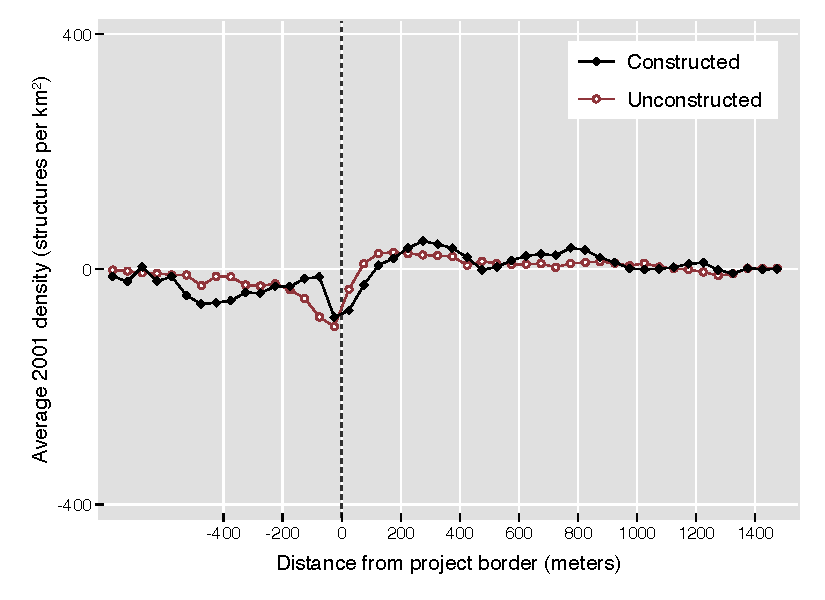
\includegraphics[width=\textwidth,trim={0.3cm .3cm 0.1cm 0cm}, clip=true]{figures/bblu_for_pre_means_4_10k.pdf}
            \caption[Network2]%
            {{\small pre-period formal housing density}}    
            \label{fig:prefor}
        \end{subfigure}
        \hfill
        \begin{subfigure}[b]{0.495\textwidth}  
            \centering 
            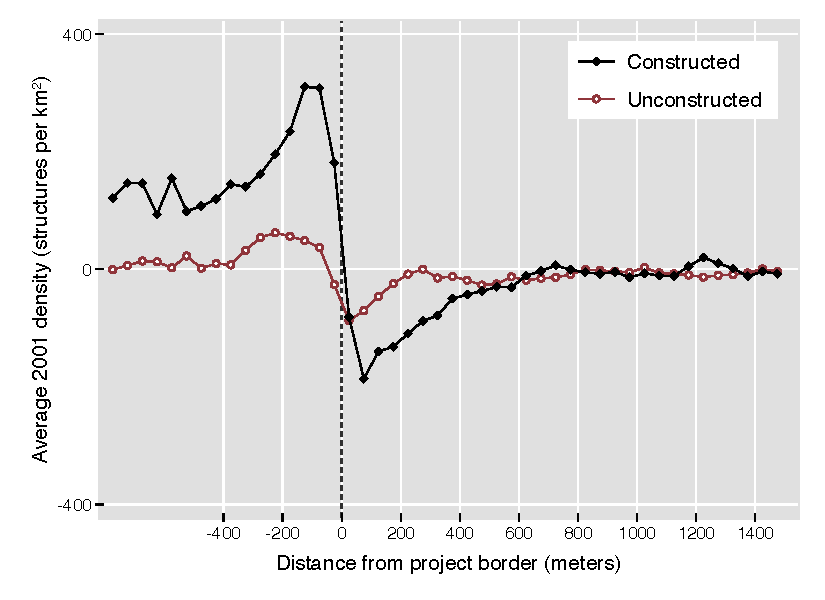
\includegraphics[width=\textwidth,trim={0.3cm .3cm 0.1cm 0cm}, clip=true]{figures/bblu_inf_pre_means_4_10k.pdf}
            \caption[]%
            {{\small pre-period informal housing density}}    
            \label{fig:preinf}
        \end{subfigure}
        \label{fig:rawbblumeans}
        \vspace{-6mm}
        \centering
        \caption[ Changes in Housing Densities in Constructed and Unconstructed Projects Areas]
        {\small 1km Square Fixed Effects (400 grid cells within) Housing Densities in Constructed and Unconstructed projects } 
        %\vspace{2mm}
        \begin{subfigure}[b]{0.495\textwidth}   
            \centering 
            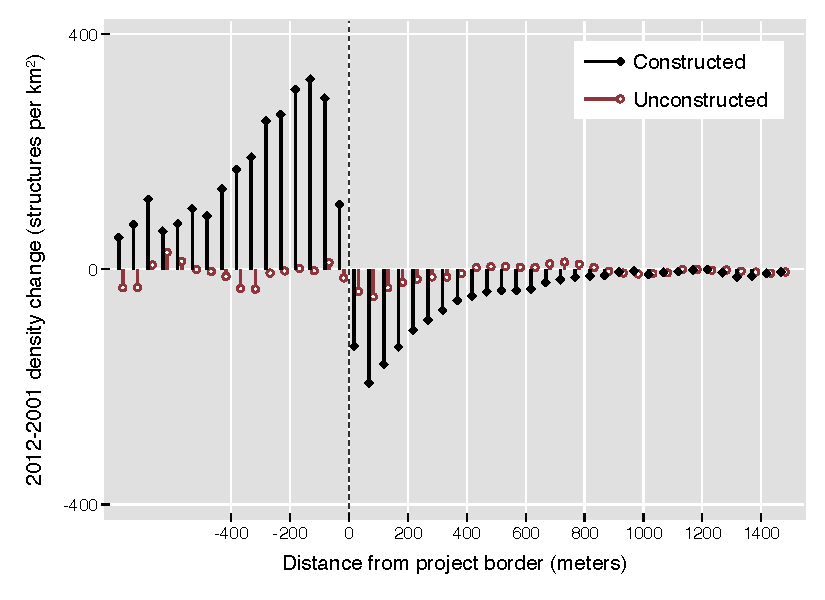
\includegraphics[width=\textwidth,trim={0.3cm .3cm 0.1cm 0cm}, clip=true]{figures/bblu_for_rawchanges_4_10k.pdf}
            \caption[]%
            {{\small formal housing density change}}    
            \label{fig:forchange}
        \end{subfigure}
        \hfill
        \begin{subfigure}[b]{0.495\textwidth}   
            \centering 
            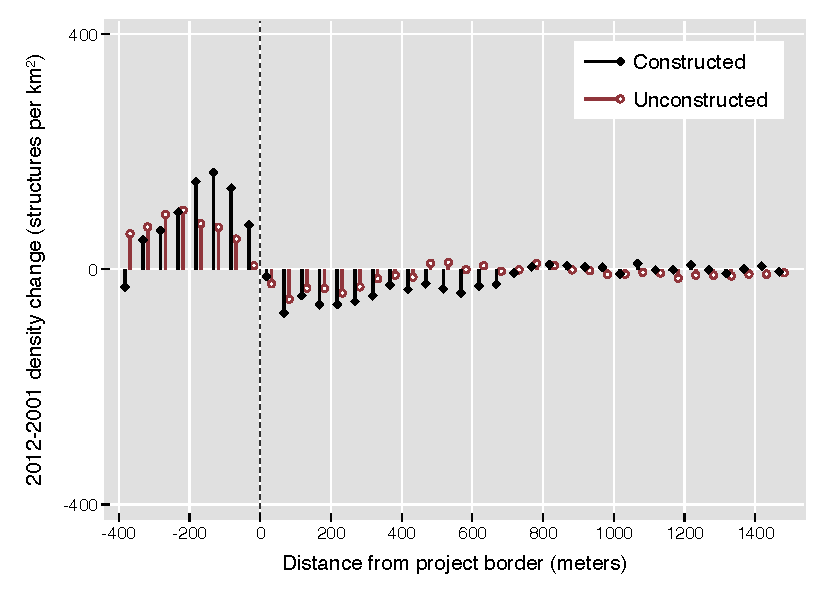
\includegraphics[width=\textwidth,trim={0.3cm .3cm 0.1cm 0cm}, clip=true]{figures/bblu_inf_rawchanges_4_10k.pdf}
            \caption[]%
            {{\small informal housing density change}}    
            \label{fig:infchange}
        \end{subfigure}
        \label{fig:rawbblumeanschange}
        \vspace{-6mm}
    \end{figure*} 




\begin{figure*}[h!]
        \centering
        \caption[ Pre-Period Housing Densities in Constructed and Unconstructed Projects Areas ]
        {\small around 20,000 0.5km Square Fixed Effects, each with 100 grid cells within  Pre-Period Housing Densities in Constructed and Unconstructed projects } 
        %\vspace{2mm}
        \begin{subfigure}[b]{0.495\textwidth}
            \centering
            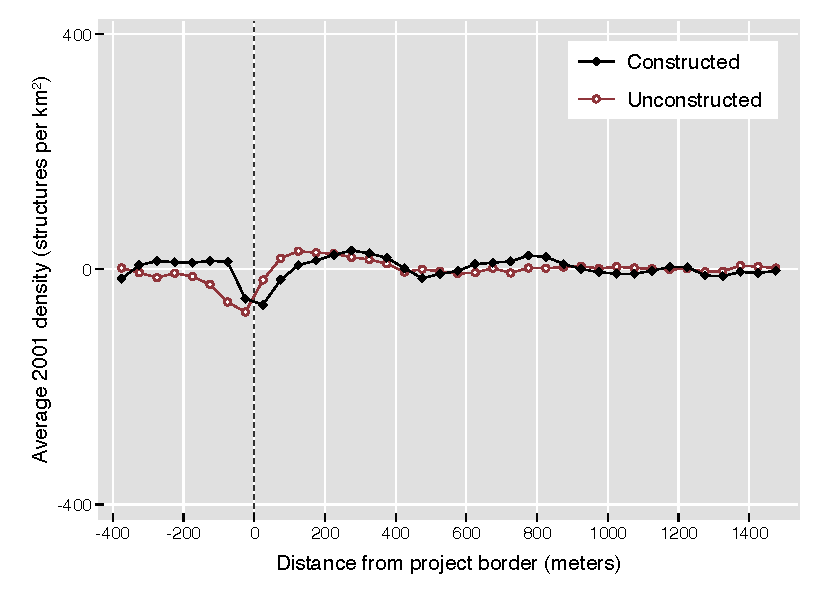
\includegraphics[width=\textwidth,trim={0.3cm .3cm 0.1cm 0cm}, clip=true]{figures/bblu_for_pre_means_4_5k.pdf}
            \caption[Network2]%
            {{\small pre-period formal housing density}}    
            \label{fig:prefor}
        \end{subfigure}
        \hfill
        \begin{subfigure}[b]{0.495\textwidth}  
            \centering 
            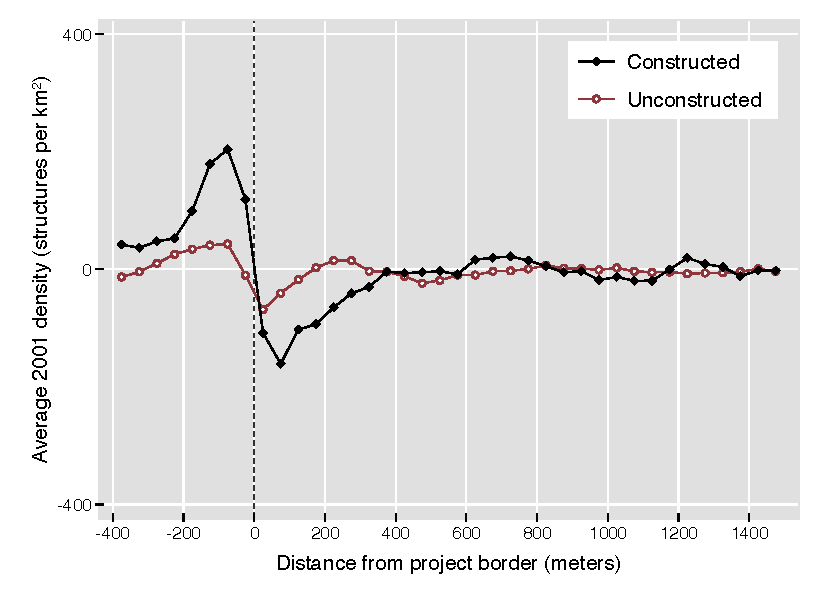
\includegraphics[width=\textwidth,trim={0.3cm .3cm 0.1cm 0cm}, clip=true]{figures/bblu_inf_pre_means_4_5k.pdf}
            \caption[]%
            {{\small pre-period informal housing density}}    
            \label{fig:preinf}
        \end{subfigure}
        \label{fig:rawbblumeans}
        \vspace{-6mm}
        \centering
        \caption[ Changes in Housing Densities in Constructed and Unconstructed Projects Areas]
        {\small 0.5km Square Fixed Effects (100 grid cells within)  Housing Densities in Constructed and Unconstructed projects } 
        %\vspace{2mm}
        \begin{subfigure}[b]{0.495\textwidth}   
            \centering 
            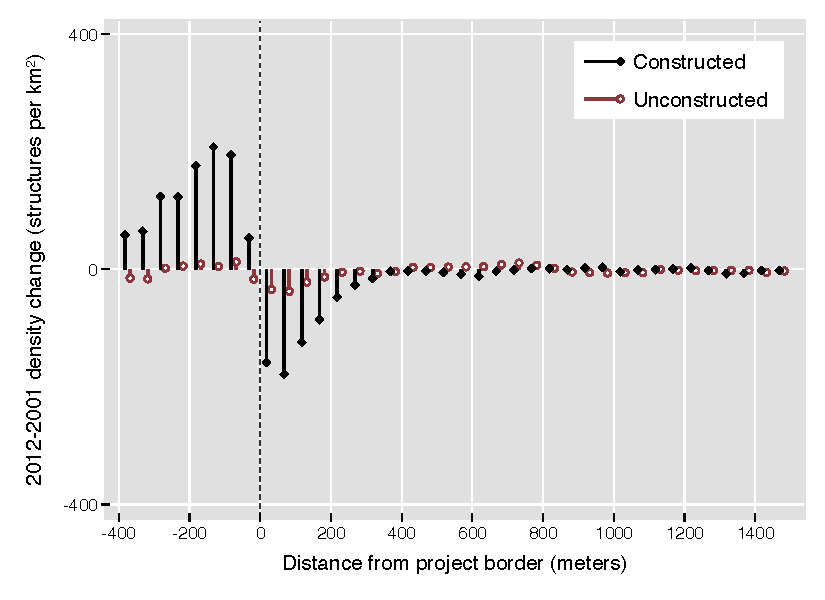
\includegraphics[width=\textwidth,trim={0.3cm .3cm 0.1cm 0cm}, clip=true]{figures/bblu_for_rawchanges_4_5k.pdf}
            \caption[]%
            {{\small formal housing density change}}    
            \label{fig:forchange}
        \end{subfigure}
        \hfill
        \begin{subfigure}[b]{0.495\textwidth}   
            \centering 
            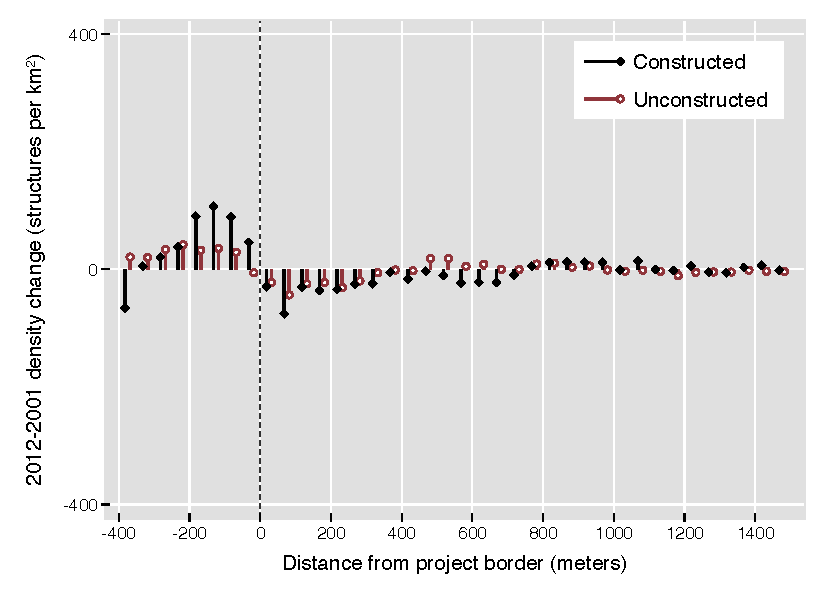
\includegraphics[width=\textwidth,trim={0.3cm .3cm 0.1cm 0cm}, clip=true]{figures/bblu_inf_rawchanges_4_5k.pdf}
            \caption[]%
            {{\small informal housing density change}}    
            \label{fig:infchange}
        \end{subfigure}
        \label{fig:rawbblumeanschange}
        \vspace{-6mm}
    \end{figure*} 



\end{document}


